\documentclass[11pt]{article}
\usepackage[utf8]{inputenc}
\usepackage[a4paper,margin=1.0in]{geometry}
\usepackage{amsmath,amssymb,amsthm}
\usepackage{bm}       % Added for bold math vectors/matrices
\usepackage{graphicx} % Added for figure rendering

%\linespread{1.15}
\linespread{2.0} % double space (BMC Medical Research Methodology)

\begin{document}
\setcounter{section}{1} % Forces the following \section to be numbered 2

% --- METHODS (theory) ---
\section{Theoretical Methods}

\subsection{Study Region and Spatial Structure}

To formalize the spatial relationships inherent in a cluster randomized trial (CRT), the theoretical study region is defined as a regular square lattice grid. Let the spatial domain be denoted as $\mathcal{G} = \{s_1, s_2, \dots, s_N\}$, where each spatial cluster $s_i$ is located at discrete integer coordinates $(x_i, y_i)$. The total number of uniformly sized clusters within the geographic network is $N$. Utilizing a regular lattice structure isolates the methodological evaluation of the sampling designs from the confounding effects of irregular polygon geometries and heterogeneous cluster populations, providing a standardized baseline to systematically compare trial designs \cite{cressie_statistics_1993}.

The spatial relationships between clusters are parameterized using strict contiguity-based definitions, which dictate the pathways through which intervention effects and spatial dependence propagate. Two primary contiguity structures are formalized for this framework:

\begin{enumerate}
    \item \textbf{Rook Contiguity:} Clusters are considered adjacent neighbors strictly if they share a direct horizontal or vertical edge. The neighborhood set for a given cluster $s_i$ under Rook contiguity is defined as:
    \begin{equation}
        \mathcal{N}_R(s_i) = \left\{ s_j \in \mathcal{G} : |x_i - x_j| + |y_i - y_j| = 1 \right\}
    \end{equation}
    
    \item \textbf{Queen Contiguity:} Clusters are considered neighbors if they share either a direct edge or a single vertex, inherently including diagonal adjacencies. The corresponding neighborhood set is defined as:
    \begin{equation}
        \mathcal{N}_Q(s_i) = \left\{ s_j \in \mathcal{G} : \max(|x_i - x_j|, |y_i - y_j|) = 1 \right\}
    \end{equation}
\end{enumerate}

To incorporate these neighborhood structures into the spatial econometric modeling, an $N \times N$ spatial weight matrix, $\bm{W}$, is constructed \cite{lesage_introduction_2009}. Let $\bm{A}$ denote an $N \times N$ binary adjacency matrix where the element $A_{ij} = 1$ if $s_j \in \mathcal{N}(s_i)$, and $A_{ij} = 0$ otherwise. By convention, $A_{ii} = 0$ for all $i$. It is important to note that clusters located on the boundaries of the spatial grid naturally possess fewer neighbors (edge effects). To facilitate the interpretation of spatial lags as localized neighborhood averages, the weight matrix $\bm{W}$ is row-standardized. This row-standardization inherently compensates for these edge effects by distributing the total weight equally among the available neighbors, rather than assuming a torus (wrap-around) grid structure. The elements of the row-standardized spatial weight matrix are strictly defined as:
\begin{equation}
    W_{ij} = \frac{A_{ij}}{\sum_{k=1}^N A_{ik}} \quad \text{for } i \neq j, \text{ and } W_{ii} = 0
\end{equation}

\subsection{Data Generating Process and the Spatial Durbin Model}

In community-based public health trials, the observed outcome within a specific geographic cluster is rarely independent of its surrounding spatial context. To capture both the endogenous spatial dependence of the outcome variable and the exogenous spillover effects generated by the localized treatment, the data-generating process utilizes the Spatial Durbin Model (SDM) \cite{lesage_introduction_2009}. The continuous outcome vector for the spatial grid, $\bm{Y} = (Y_1, \dots, Y_N)^\top$, is expressed in its reduced structural form as:
\begin{equation}
    \bm{Y} = (\bm{I}_N - \rho \bm{W})^{-1} [\tau \bm{Z} + \gamma \cdot \text{Spill}(\bm{Z}) + \beta \bm{X} + \bm{\epsilon}]
\end{equation}

In this structural equation, the parameters operate as follows:
\begin{itemize}
    \item $\bm{I}_N$ is the $N \times N$ identity matrix.
    \item $(\bm{I}_N - \rho \bm{W})^{-1}$ acts as the global spatial multiplier. This multiplier induces global spatial dependence, ensuring that a localized intervention effect reverberates throughout the entire spatial network, decaying exponentially with topological distance.
    \item $\rho$ is the spatial autocorrelation coefficient. The condition $|\rho| < 1$ must be maintained to ensure the matrix is invertible and the spatial process remains stable.
    \item $\tau$ is the primary estimand of interest, representing the true direct effect of the intervention on the treated cluster.
    \item $\bm{Z}$ is an $N \times 1$ binary treatment assignment vector, where $Z_i = 1$ indicates that cluster $s_i$ received the active intervention.
    \item $\bm{X}$ is an $N \times 1$ continuous vector representing the pre-existing baseline outcome incidence within each cluster.
    \item $\beta$ is a scalar coefficient governing the direct linear effect of the baseline incidence $\bm{X}$ on the final observed outcome.
    \item $\bm{\epsilon}$ represents an $N \times 1$ vector of independent and identically distributed random error terms, where $\bm{\epsilon} \sim \mathcal{N}(\bm{0}, \sigma^2 \bm{I}_N)$.
\end{itemize}

The function $\text{Spill}(\bm{Z})$ calculates an $N \times 1$ vector representing the degree of indirect treatment exposure that each cluster receives from its immediate neighbors, weighted by the scalar spillover magnitude parameter, $\gamma$. The base spillover exposure for a given cluster $i$ is calculated as the proportion of its contiguous neighbors assigned to the intervention arm: $(\bm{W}\bm{Z})_i = \frac{1}{|\mathcal{N}(i)|} \sum_{j \in \mathcal{N}(i)} Z_j$. This specification explicitly assumes an additive, proportional interference mechanism common in community-level interventions, rather than a threshold-based interference model.

This framework accommodates two mathematical mechanisms of spillover propagation:
\begin{enumerate}
    \item \textbf{Bidirectional Spillover (Intervention \& Control):} The indirect spillover effect impacts all clusters in the network regardless of their internal treatment assignment status. The exposure for cluster $i$ is defined as $\text{Spill}_i^{(both)} = (\bm{W}\bm{Z})_i$.
    \item \textbf{Control-Only Spillover:} The spillover effect functions exclusively as an externality for clusters that did not directly receive the intervention. Once a cluster is actively treated, its outcome cannot be further improved by neighboring treatments. The exposure is defined using a Hadamard product to mathematically mask treated units: $\text{Spill}_i^{(ctrl)} = (\bm{W}\bm{Z})_i \cdot (1 - Z_i)$.
\end{enumerate}

\subsection{Spatially Heterogeneous Incidence Generation}

The baseline incidence vector $\bm{X}$ models the historical, pre-intervention outcome rates distributed across the geographic clusters. To rigorously evaluate the vulnerability of spatial sampling designs to underlying data structures, $\bm{X}$ is generated via three distinct modes. The final incidence metric $X_i$ is computationally mapped to a strictly continuous scale bounded within $[0, 1]$. Mapping the incidence to this standardized interval ensures that the coefficient $\beta$ maintains a consistent relative magnitude of impact across all three structurally diverse data generation processes.

\textbf{Mode 1: Independent and Identically Distributed (iid) Uniform Incidence}\\
As a methodological baseline, incidence is generated with no underlying spatial structure. For each cluster $i$:
\begin{equation}
    X_i \sim \text{Uniform}(0, 1) \quad \text{for } i = 1, \dots, N
\end{equation}

\textbf{Mode 2: Spatially Correlated Incidence (SAR Filter)}\\
To reflect scenarios where underlying outcomes naturally cluster geographically, incidence is generated utilizing a Simultaneous Autoregressive (SAR) filter \cite{lesage_introduction_2009}. A spatially correlated continuous variable is constructed:
\begin{equation}
    \bm{X}^* = (\bm{I}_N - \rho_X \bm{W})^{-1} \bm{u}, \quad \text{where } \bm{u} \sim \mathcal{N}(\bm{0}, \bm{I}_N)
\end{equation}
Here, $\rho_X \in [0, 1)$ controls the degree of spatial autocorrelation strictly within the baseline incidence. A probability integral transform is applied using the standard normal cumulative distribution function, $\Phi(\cdot)$, yielding the final bounded incidence: $X_i = \Phi(X_i^*)$.

\textbf{Mode 3: Poisson Count-Based Incidence}\\
Motivated by empirical disease incidence distributions---specifically Sudden Unexpected Death (SUD) demographic data \cite{mirzaei_years_2019, gan_factors_2019}---this mode generates discrete event counts based on localized population densities and spatially correlated underlying relative risks. First, spatially correlated log-rates, $\log \bm{\lambda}^*$, are generated relative to a global base rate, $\mu_0$:
\begin{equation}
    \log \bm{\lambda}^* = \mu_0 \bm{1} + (\bm{I}_N - \rho_X \bm{W})^{-1} \bm{u}, \quad \text{where } \bm{u} \sim \mathcal{N}(\bm{0}, \bm{I}_N)
\end{equation}
Expected case counts, $C_i$, are subsequently drawn from a Poisson distribution scaled by the discrete population of the cluster, $P_i$:
\begin{equation}
    C_i \sim \text{Poisson}(\lambda_i^* P_i)
\end{equation}
The observed raw rates are calculated as $R_i = C_i / P_i$. These rates are rank-normalized to preserve ordinal spatial clustering while mapping the final values strictly to the uniform $[0, 1]$ interval: 
\begin{equation}
    X_i = \frac{\text{rank}(R_i) - 0.5}{N}
\end{equation}

\subsection{Treatment Assignment Designs}

The explicit determination of the binary treatment vector $\bm{Z}$ dictates how the direct intervention is deployed across the targeted region. This methodology contrasts strictly spatial randomization methods against covariate-constrained assignment algorithms that actively utilize the observed incidence vector $\bm{X}$. Each sampling design targets a globally balanced allocation where approximately half of the clusters receive the intervention ($\sum_{i=1}^N Z_i \approx N/2$).

\begin{figure}[htbp]
  \centering
  % Uncomment the line below and remove the \rule in your actual Overleaf document
  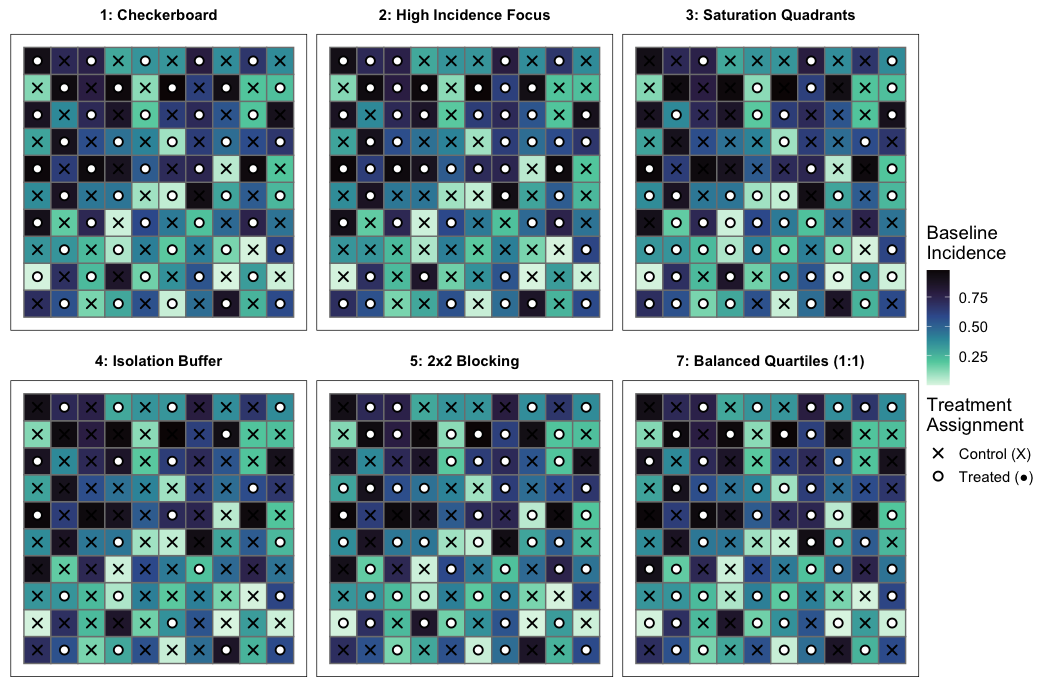
\includegraphics[width=0.9\textwidth]{figures/SamplingGridExamples_crop.png}
  \caption{A grid of visualizations displaying one realization of each of the six treatment assignment designs overlaid on a standard $10 \times 10$ spatial grid. Dark circular markers indicate clusters assigned to the intervention arm ($Z_i=1$), while cross markers indicate control clusters ($Z_i=0$). The underlying continuous color gradient represents the baseline incidence distribution ($\bm{X}$).}
  \label{fig:sampling_designs}
\end{figure}

\subsubsection{Strictly Spatial Methods}
\begin{enumerate}
    \item \textbf{Block Stratification:} A deterministic, alternating assignment pattern designed to maximize spatial separation by ensuring that every treated cluster is entirely surrounded by control clusters under Rook contiguity. Mathematically, for a cluster at coordinates $(x_i, y_i)$, the assignment is $Z_i = (x_i + y_i) \pmod 2$.
    \item \textbf{$2 \times 2$ Random Blocking:} The global spatial lattice is evenly partitioned into distinct, non-overlapping $2 \times 2$ contiguous geographic blocks. Within each localized block of four clusters, exactly two clusters are stochastically assigned to the intervention arm. 
    \item \textbf{Isolation Buffer Treatment Clusters:} A stochastic, greedy spatial algorithm designed to entirely prevent contiguous treatment spillover between active intervention units. An available cluster is randomly selected for treatment ($Z_i = 1$). Immediately following selection, that specific cluster and all of its immediate contiguous neighbors are permanently removed from the eligible assignment pool. 
\end{enumerate}

\subsubsection{Covariate-Constrained Methods (Incidence-Guided)}
\begin{enumerate}
    \setcounter{enumi}{3}
    \item \textbf{Median Incidence Grouping:} A deterministic allocation strategy that actively targets the geographic areas suffering from the highest historical burden. Clusters are assigned to the intervention arm strictly if their baseline incidence exceeds the median of the global incidence distribution. Formally, $Z_i = 1$ if $X_i > \text{median}(\bm{X})$, and $Z_i = 0$ otherwise.
    \item \textbf{Saturation Quadrants:} The spatial grid is bisected along both axes, partitioning the landscape into four equally sized geographic quadrants. Each quadrant is randomly assigned a distinct, fixed treatment saturation density without replacement (e.g., exactly 20\%, 40\%, 60\%, and 80\% treated). Clusters are randomly assigned to the intervention arm until the localized saturation target is met.
    \item \textbf{Treatment Balanced Incidence Quartiles:} Clusters are initially stratified into four continuous strata strictly based on the calculated quartiles of the baseline incidence vector $\bm{X}$. Within each unique incidence stratum, exactly 50\% of the clusters are randomly assigned to the intervention arm, balancing the historical severity of the outcome across both the treatment and control groups.
\end{enumerate}

\subsection{Estimation via Maximum Likelihood}

In the presence of endogenous spatial dependence ($\rho \neq 0$) and exogenous spillover ($\gamma \neq 0$), estimators such as the Difference-in-Means fundamentally violate the Stable Unit Treatment Value Assumption (SUTVA). Furthermore, Ordinary Least Squares (OLS) regression fails as an unbiased estimator in this context due to continuous spatial feedback loops. Because the unobserved spatial structure correlates simultaneously with both the treatment assignment mechanics and the final outcome, the expected value of the error term conditional on the regressors is non-zero ($E[\bm{\epsilon} \mid \bm{Z}, \bm{W}] \neq 0$). Consequently, OLS models suffer from simultaneity bias, yielding systematically biased point estimates and artificially deflated standard errors.

To achieve statistically consistent estimation of the direct intervention effect $\tau$, a spatial autoregressive regression framework must be utilized \cite{bivand_comparing_2015}. The corresponding empirical estimation model takes the matrix form:
\begin{equation}
    \bm{Y} = \rho \bm{W} \bm{Y} + \bm{X}_{design}\bm{\beta}_{design} + \bm{\epsilon}
\end{equation}
Where the composite design matrix is horizontally concatenated as $\bm{X}_{design} = [\bm{Z} \quad \text{Spill}(\bm{Z}) \quad \bm{X}]$ and the corresponding vector of coefficients to be estimated is $\bm{\beta}_{design} = (\tau, \gamma, \beta)^\top$. 

Because the response variable $\bm{Y}$ inherently appears on both sides of the structural equation, the parameters must be estimated simultaneously via concentrated Maximum Likelihood Estimation (MLE). This approach optimizes a log-likelihood function that explicitly incorporates the Jacobian determinant of the spatial transformation, $\ln|\bm{I}_N - \rho \bm{W}|$. This term evaluates the likelihood space and partitions the variance by concurrently estimating the spatial autocorrelation parameter alongside the direct and indirect treatment coefficients. The theoretical integration of incidence-guided sampling algorithms with spatial MLE is evaluated to determine optimal frameworks for causal inference in complex spatial environments.

% --- BIBLIOGRAPHY (from Zotero) ---
% sample citations

% print bibliography
%\bibliographystyle{plain} % alphabetical order
\bibliographystyle{unsrt} % order of appearance
\bibliography{references.bib}
\end{document}